In this chapter we summarize the main results of the thesis. Section~\ref{sec:concl_glitch} reviews the work presented in Chapters~\ref{chap:acorr}--\ref{chap:hda}, in which we attempt to falsify various underlying mechanisms which may cause pulsar glitches, by understanding the long-term statistical predictions of phenomenological stress-accumulation and relaxation meta-models, and comparing to observations. In Section~\ref{sec:concl_sf} we review the application of one such meta-model to solar flares, as discussed in Chapter~\ref{chap:sf}. Section~\ref{sec:concl_amxp} reviews the search for continuous gravitational waves from AMXPs in O3 LIGO data, as presented in Chapter~\ref{chap:amxp}. We sketch various avenues for future work throughout.

\section[Understanding pulsar glitches through the lens of stress- \linebreak accumulation and relaxation meta-models]{Understanding pulsar glitches through the lens of stress-accumulation and relaxation meta-models} \label{sec:concl_glitch}
What causes pulsar glitches is unknown. There are numerous physical mechanisms popular in the literature (see \citet{Haskell2015,Antonopoulou2022,Antonelli2022,Zhou2022} for modern reviews). Almost all of these mechanisms are, at an abstract level, stress-accumulation and relaxation processes. That is, while the glitch trigger mechanism varies, there is broad agreement that stress accumulates in the pulsar between glitches, and some of this stress is released at each glitch.

The state-dependent Poisson (SDP) process is a doubly-stochastic system, wherein a globally-averaged stress $X$ is tracked as a function of time. The waiting times $\Delta t$ between stress-release events are random, but events become more likely as $X$ approaches the critical stress $\xc$, at which point a stress-release event becomes certain. The speed at which the system is driven towards $\xc$ is determined by the control parameter $\alpha$. The amount of stress released at each event is another random variable, and is governed by the conditional jump-size distribution $\etadx$. This distribution is determined by fiat, and can be treated as a free parameter in the meta-model, or it can encode one's belief regarding the underlying physical mechanism. For example, if $\eta$ is a power law, the amount of stress released at each event is scale-free, which is a hallmark of an avalanche-type process. While keeping $\eta$ as a free parameter, the SDP framework can successfully and self-consistently generate sequences of glitch waiting times, sizes, and cross-correlations thereof which match those from the most-glitching pulsars \citep{Fulgenzi2017,Melatos2018,Carlin2019quasi}. The SDP process is a broad framework, that encompasses many, but not all, microphysical trigger mechanisms. To test, and potentially falsify, specific mechanisms we adapt and probe the SDP framework in different ways in this thesis.

In Chapter~\ref{chap:acorr} we investigate the autocorrelation between subsequent waiting times $\rho_{\Delta t}$, or subsequent sizes $\rho_{\Delta X}$. These are long-term statistical quantities easily calculable in the SDP framework, and measurable from glitch observations. We find that most configurations of the SDP process, i.e.~combinations $\eta$ and $\alpha$, result in autocorrelations that are consistent with zero. However, there are certain regimes that are ruled out. For example, if $\eta$ is a Gaussian, we always have $\rho_{\Delta t} \leq 0$. The waiting times, sizes and cross-correlations of the quasiperiodic glitching pulsar PSR J0537$-$6910 are only consistent with the SDP process if we have $\eta$ unimodal and $\alpha \lesssim 10^{-2}$. Thus, if we detected $\rho_{\Delta t} > 0$ in this pulsar, we would falsify the SDP process. We find $\rho_{\Delta t} \lesssim 0$. We also find configurations of $\eta$ and $\alpha$ that can simultaneously explain the observed waiting time and size PDFs \citep{Carlin2019quasi}, cross-correlations \citep{Melatos2018}, and autocorrelations \citep{Carlin2019ac} in all other glitching pulsars that have enough recorded glitches to make such measurements. That is, we cannot currently falsify the SDP process in any glitching pulsar. However, this may change as more glitches are discovered, both in historic datasets \citep{Basu2022,Dunn2022,Dunn2023}, and through continued monitoring of known pulsars \citep{Jankowski2019,Basu2020,Johnston2020,Amiri2021}. 

In Chapter~\ref{chap:bsa} we explore the impact that a stochastic stress driver has on long-term statistical predictions. A stochastic driver may be connected to timing noise (see Section~\ref{sec:intro_tn}) or superfluid turbulence \citep{Melatos2007,Melatos2014,Khomenko2019}. By replacing the secular intra-glitch evolution of the stress with a stochastic process, we in turn require that the stress reach a threshold before each event is triggered. The waiting times between events depend on how much stress was released at the previous event, and the balance between drift and diffusion in the Brownian walk of the stress. As for the SDP framework, we make precise, falsifiable predictions regarding what combinations of long-term statistical observables are possible to generate within the Brownian stress accumulation meta-model. When we compare these predictions to pulsar data, we find the meta-model is falsified in at least some pulsars. For example PSR J0534+2200 has a very low forward cross-correlation, which can only be generated from the meta-model if diffusion dominates over drift in the Brownian random walk. In this regime, we should see an excess of events with very small waiting times, however there is no evidence of such in the data. Therefore, unless we are missing many glitches with $\Delta t \lesssim 0.25 \langle \Delta t \rangle$, this meta-model cannot explain all glitches from all pulsars.

The final glitch meta-model we investigate in this thesis returns to the SDP framework, but prescribes the size of stress-release events endogenously. In Chapter~\ref{chap:hda} we assume pulsar glitches are caused by superfluid vortex avalanches, triggered via a coherent stress mechanism. Under this assumption, we codify the current understanding of the microphysical rules regarding how vortices pin and unpin, to phenomenologically track the pinning strength of pinning sites that are occupied, as a function of time. Doing so allows us to know what fraction of vortices unpin once a stress-release event is triggered, i.e.~the size of stress-release events is no longer a random variable, but is instead determined by the history of past avalanches in the system. This meta-model again makes precise, falsifiable predictions regarding combinations of long-term statistical observables. We find these predictions broadly inconsistent with observational data from most glitching pulsars, provisionally falsifying the meta-model. This does not imply that glitches must be caused by a mechanism other than superfluid vortex avalanches. The meta-model idealizes much of the detailed microphysics. Simulations suggest that spatial correlations play a key role in vortex motion \citep{Howitt2020}, while the coherent stress mechanism addressed here assumes one, globally-averaged stress is felt at all pinning sites.

One limiting factor in drawing concrete conclusions from glitch meta-models is the paucity of data. As seen in Table~\ref{tab:glitch_stats}, only six pulsars have more than 15 recorded glitches. \citet{Millhouse2022, Melatos2023glitch} use even the non-detection of glitches to estimate glitch rates across the population of pulsars, and by implementing a hierarchical Bayesian scheme, estimate various SDP parameters. However, the analysis in the aforementioned papers does not incorporate glitch sizes, or long-term observables such as cross- or autocorrelations. Incorporating this additional information is not trivial, as it would result in fitting a complicated, non-convex likelihood to the data \citep{Melatos2019}. A reformulation of stress-relax meta-models into the mathematical language of jump-diffusion processes might unlock optimal filtration techniques (e.g.~the Kushner and Zakai equations \citep{Kushner1964,Zakai1969}), allowing us to optimally estimate parameters of the process given noisy, sparse measurements \citep{Schuss2012}.

Detecting more glitches is possible via a combination of: \begin{enumerate*}
\item observing known glitching pulsars with a higher cadence;
\item observing known glitching pulsars with a longer dwell time, or higher sensitivity;
\item applying and developing more sensitive glitch detection algorithms; and/or
\item finding more pulsars which glitch.
\end{enumerate*}
Point (i) will allow for earlier detection of glitches, and the detection of smaller glitches with fast recoveries (i.e.~glitches that with a longer cadence may not have a noticeable impact on the timing solution). Relatedly, a higher cadence will also allow for easier discrimination between timing noise and small glitches \citep{Melatos2020hmm, Dunn2022}, something that point (ii) will also assist with. Point (iii) is an ongoing area of research \citep{Lentati2014,Melatos2020hmm,Singha2021a}. Sensitive future facilities, such as the Square Kilometer Array, will allow for the discovery and continuous monitoring of many more glitching pulsars than are currently known \citep{Watts2015, Singha2022}. That is, they will assist points (ii) and (iv). However, unless the proposed fortnightly cadence of observations is reduced, these future facilities will not help us accurately determine the low end of the glitch size or waiting time distribution, which is crucial for distinguishing between the meta-models discussed in Chapters~\ref{chap:acorr}--\ref{chap:hda}. 

A natural question remains: how many glitches will we need to detect before we can confidently discriminate between different meta-models? This is non-trivial to answer quantitatively. Appendix B of \citet{Melatos2019} approaches this question in terms of how many glitches are needed before the SDP meta-model can more accurately predict future glitch epochs, compared to a simple Poisson process, assuming glitches truly arise from the SDP process. They find that at least 50, and up to hundreds of glitches are necessary. However, if certain pulsars are found to have, for example, a waiting time or size autocorrelation statistically different from zero, certain meta-models (such as the one discussed in Chapter~\ref{chap:bsa}) are immediately disfavored. This could occur with as few as $\sim30$ glitches, dependent on the true underlying autocorrelation (c.f.~Equation~\eqref{eq:ac_rhoci}). 

\section{Are solar flares the result of stress approaching a threshold before each event?} \label{sec:concl_sf}
In Chapter~\ref{chap:sf} we turn our attention to solar flares. The typical explanation for flares is that subphotospheric, convective motion transports energy into the magnetic field of the corona. This energy accumulates over time, and releases suddenly when the footpoints of coronal loops or arcades shift, triggering a reconnection event \citep{Priest2002,Benz2016}. Accordingly, there is a long history of building phenomenological stress-relax models that track this energy and predict statistical signatures \citep{Rosner1978,Wheatland1998,Wheatland2000corr,Wheatland2008,Hudson2019}. One such signature is a cross-correlation, $\rho_+$, between size of a flare and the subsequent waiting time. We should see a large $\rho_+$, if the stress threshold does not vary from flare to flare, and the stress reaches this threshold before every flare. Searches for statistical signatures of these models in data has a similarly long history \citep{Gaizauskas1987,Biesecker1994,Crosby1998,Hudson1998,Hudson2019,Hudson2020}. However, barring a few exceptions \citep{Ellison1963,Hudson2019}, the vast majority of these studies do not find any evidence of a large $\rho_+$, nor evidence of a static-in-time threshold. For example, in summarizing the Flare Build-Up Study, \citet{Gaizauskas1987} state that there is ``no consistent relationship [...] between the repetition rate of homologous flares and their X-ray [...] brightness'' (verbatim quote).
 
An alternative set of phenomenological models in the literature posits solar flares as analogous to systems in a state of self-organized criticality, such as sandpiles or avalanches, in which case there should exist no cross-correlations between sizes and waiting times, and one should see a power law size PDF \citep{Parker1988,Lu1991,Lu1995,Charbonneau2001}. The SDP framework broadly encompasses both sets of phenomenological models. If we have $\alpha \ll 1$ the process is threshold-driven, i.e.~approaches a static-in-time threshold before each event. On the other hand, for $\alpha \gg 1$, there is little long-term memory in the system, and the dynamics are largely determined by the choice of $\eta$, which can be fixed as a power law, producing a power law size PDF.

We analyze the \emph{GOES} soft X-ray flare dataset, which contains over $8\times10^5$ events. We look for statistical signatures of a SDP process in sequences of flare sizes and waiting times in individual active regions. For example, we investigate whether the flare rate $\lambda_k$ (a potential proxy for $\alpha$) is associated with larger $\rho_+$, and find a small but non-zero Spearman correlation of $5\times10^{-2}$ (p-value of 0.06), see Figure \ref{fig:sf_hist_corr}. Another test is to see whether the regions which have similar waiting time and size PDFs also have large $\rho_+$, another key prediction of the SDP framework if we have $\alpha \ll 1$. We see no evidence for this association in the \emph{GOES} data, see Figure~\ref{fig:sf_goes_kde}. These results are predicated on the completeness of the flare catalog, which is not guaranteed, as discussed in detail in Section~\ref{sec:sf_obscuration}. We find no strong evidence that flares are the result of a SDP process in the $\alpha \ll 1$ regime, where stress approaches a static-in-time threshold before every flare. However, the SDP process assumes that stress is driven into the system at a constant rate, and that the threshold does not vary from flare to flare. Alternative meta-models may soften these assumptions in the future. 

There are many open questions regarding the physics behind solar flares that can be guided by the SDP framework. For example, one may look for a correlation between statistical measurements that are directly linked to SDP predictions or input parameters, such as $\rho_+$ or $\lambda_k$ respectively, with other observables for a given active region. This regression should at minimum include the phase of the solar cycle, as a proxy for the Sun's large-scale magnetic field strength \citep{Hathaway2015}, the morphology of the active region \citep{Abramenko2023}, and vector magnetogram estimates of both the perpendicular and line-of-sight magnetic field strength in the active region \citep{Bobra2015,Abramenko2017}. Such an exercise could help untangle the potential causal links between the physical properties of the active region, and the SDP parameters that govern the statistical behavior of flare occurrence. Estimating SDP parameters in individual regions may also lead to an improvement in our ability to predict flares, although this will likely only be possible in regions that already have many flares observed, see Appendix B of \citet{Melatos2019} for an exploration of this possibility in the context of pulsar glitch epoch prediction. Flare prediction using purely data-driven algorithms is difficult \citep{Barnes2016,Leka2019,Leka2019a}, but astrophysically motivated models can help in some circumstances \citep{Thibeault2022}.

\section[Searching for continuous gravitational waves from accreting millisecond X-ray pulsars]{Searching for continuous gravitational waves \linebreak from accreting millisecond X-ray pulsars} \label{sec:concl_amxp}
Despite much effort, continuous gravitational waves are yet to be detected. Detecting a small signal in noise requires an accurate signal model. Continuous gravitational wave searches for neutron stars in binary systems, such as AMXPs, require us to model not just the deterministic evolution of the gravitational wave frequency, but also allow for some degree of stochastic variation due to spin-wandering. In Chapter~\ref{chap:amxp}, we use the $\mj$-statistic \citep{Suvorova2017} as a matched filter for the signal over coherent chunks of $T_{\rm drift} = 10\,$d. That is, we assume that the gravitational wave frequency stays within one frequency bin over the $10\,$d chunk, after accounting for the Doppler modulations due to Earth's motion around the solar system barycentre, as well as the target's motion in its binary. The slow stochastic variation over time is accounted for with a hidden Markov model \citep{Suvorova2016}. That is, between chunks we allow the (Doppler corrected) gravitational wave frequency to vary by up to one bin. We reconstruct the most likely path through the time--frequency trellis using the Viterbi algorithm \citep{Viterbi1967}. 

AMXPs pulsate in X-rays while they are in outburst, a period of increased X-ray flux due to an increase in mass accretion rate \citep{DiSalvo2022}. These pulsations allow for phase-coherent timing of the rotation of the neutron star, giving precise estimates for the rotation frequency and binary orbital elements. We use these precise estimates to guide our continuous gravitational wave search for 20 AMXPs. We search for gravitational waves at three $\sim0.61\,$Hz subbands, centered at once, twice, and $\sim4/3$ the spin frequency $f_\star$ of the neutron star. These harmonics are the most likely frequencies for gravitational wave emission, as discussed in Section~\ref{sec:intro_emiss}. The narrow sub-bands allow for a slight mismatch of rotation frequency between the mass quadrupole or current quadrupole that emits the gravitational waves, and the rotation frequency of the surface of the neutron star.

We find no strong evidence in LIGO O3 data for continuous gravitational waves in any subband from any of the targets. When we set a permissive false alarm probability of 30\% per subband, we find 16 candidates that survive a series of astrophysical vetoes, and we recommend that these candidates are followed up in searches using future, more sensitive datasets. We also performed an additional, target-of-opportunity search for gravitational waves from SAX J1808.4$-$3657. This target went into outburst for one month during the first half of O3, and so we search data from only that month, under the speculative hypothesis that it is only emitting gravitational waves for a short time after the outburst begins. We again find no strong evidence of a signal. Assuming all of our candidates are false alarms, we compute frequentist upper limits on the detectable strain at 95\% confidence via sequences of software injections. The lowest constraint is in the $2f_\star$ subband of IGR J17062$-$6143, where we find $h_0^{95\%} = 4.7\times10^{-26}$. Constraints on $h_0^{95\%}$ are converted to astrophysical constraints on the ellipticity $\epsilon$ and $r$-mode amplitude $\alpha$ for all targets, using Equations~\eqref{eq:amxp_ellip} and \eqref{eq:amxp_alpha} respectively. The most constraining AMXP for these quantities is IGR J00291+5934, where we find $\epsilon^{95\%} = 3.1\times10^{-7}$ and $\alpha^{95\%} = 1.8\times10^{-5}$. 

Theoretical estimates for the expected ellipticity in accreting systems vary, but current estimates for magnetically or elastically supported mountains propose $\epsilon \sim 10^{-10}$--$10^{-6}$, dependent on modelling details such as the equation of state \citep{Haskell2006,Vigelius2009,Priymak2011,Gittins2021}. Our upper limits on ellipticity therefore already provide constraints on which of these theoretical models may apply in AMXPs. Theoretical estimates for the expected $r$-mode amplitude in accreting systems propose $\alpha \sim 10^{-3}$--$10^{-4}$ \citep{Bondarescu2009, Bondarescu2013}, but are of course conditional on many unknown neutron star parameters. Again, our upper limits from AMXPs place constraints on these models. 

The upper limit we place on detectable strain depends on many factors. It is a function of the noise floor of the detector, the total observing time, choices in the signal model, and the size of the searched parameter space. The first two aspects will improve in the next observing run of the LVK, Observing Run 4 (O4). Current, publicly available information indicates that O4 will begin at the end of May 2023, and include at least 18 months of data collection, at an increased sensitivity compared to O3\footnote{\url{https://observing.docs.ligo.org/plan/}}. The improvement in sensitivity is hard to quantitatively assess while commissioning is ongoing, but a first-order estimate is possible by comparing the quoted binary neutron star (BNS) inspiral range, the distance to which a canonical binary neutron star merger is detectable with a signal-to-noise ratio of eight in a single detector. For O3, this distance was around 120\,Mpc, while in O4 it is estimated to be at least 160\,Mpc \citep{Buikema2020}. This ``range'' incorporates sensitivity improvements across a broad frequency band. The exact improvement for a continuous gravitational wave search will depend on the subband. The detectable strain scales inversely with the distance to the source, i.e.~an increase in the inspiral range corresponds to lower detectable strains, c.f.~Equation~\eqref{eq:hmunu}. That is, if the BNS range increases by a factor of $160\,\textrm{Mpc} / 120\,\textrm{Mpc} = 4/3$, we are sensitive to $3/4$ smaller strains from a source at a fixed distance. For a semi-coherent search, we have 
\begin{equation}
    h_0^{95\%} \propto (T_{\rm obs} T_{\rm drift})^{-1/4}\,, \label{eq:conc_semicoh}
\end{equation}
where $T_{\rm obs}$ is the total observing time \citep{Sun2018}. The proportionality constant in Equation~\eqref{eq:conc_semicoh} is set by the noise floor of the detectors, and the search pipeline. Detailed, individual analysis of X-ray flux variability in AMXPs may allow us to increase $T_{\rm drift}$ to (say)  $T_{\rm drift} = 20\,$d, if the stochastic variations in spin frequency are low enough \citep{Melatos2023}. 

We can further improve the detectable strain by modifying the search space. As discussed in Section~\ref{sec:amxp_numtemps}, while the orbital elements $P$, $\tasc$, and $a_0$ are precisely known from X-ray pulsation timing, we must still search over a set of templates to ensure the mismatch between the true signal parameters and those used in the search does not result in an unacceptable loss in signal-to-noise ratio. The size of the template bank feeds into the calculation for the threshold $\lth$ for a given subband, as it changes the necessary trials factor to keep the total false alarm rate at a fixed value, see Section~\ref{sec:amxp_thresh} and Appendix~\ref{app:amxp_thresh}. The $P$--$\tasc$ search space we use in Chapter~\ref{chap:amxp} conservatively covers a rectangular grid. However, the joint prior on $P$ and $\tasc$ measured electromagnetically is a multivariate Gaussian. This Gaussian has a non-diagonal covariance matrix once $\tasc$ is propagated to the start of O3. By searching a rectangular grid in $P$ and the propagated $\tasc$ we are ignoring this covariance, and search the marginal joint priors in the two parameters independently. For concreteness, we calculate this effect for the $2f_\star$ subband of Swift J175.96$-$2508. The true $3\sigma$ joint prior is shown as the purple ellipse in Figure~\ref{fig:grid_ellipse}, while the black dots mark the templates used in the O3 search. The green stars mark the O3 search templates that lie within the true joint prior. There are 24 templates within the joint prior compared to the 1340 templates we searched in O3. This indicates that we can reduce our search space by 98.2\% for this subband without any loss in probability of detection. Initial investigations indicate that comparable reductions in search space are possible in most of the other subbands. 

\begin{figure}
    \centering
    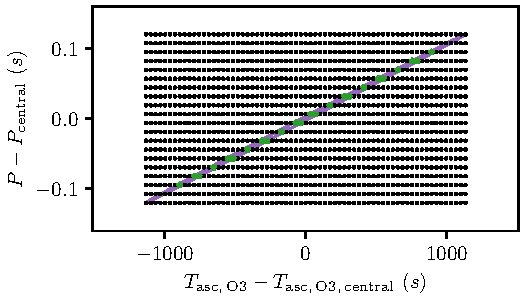
\includegraphics[width=0.8\linewidth]{swift1756_ellipse.pdf}
    \caption{Template placement in the $P$--$\tasc$ space for the $2f_\star$ subband of Swift J1756.9$-$2508. Black dots correspond to the templates in the O3 search present in Chapter~\ref{chap:amxp}. The purple ellipse is the true $3\sigma$ joint prior on these parameters, and the green crosses indicate which templates lie within this prior. $P_{\rm central}$ and $T_{\rm asc,\,central}$ refer to the central $P$ and propagated $\tasc$ values for this target, as recorded in Table~\ref{tab:info}.}
    \label{fig:grid_ellipse}
\end{figure}

One may use the optimal template placement described in \citet{Wagner2022} to further reduce the total number of templates, but this effect is minor compared to searching only the templates enclosed in the true joint prior. Another potential reduction in total templates needed is to under-sample regions of the $P$--$\tasc$ space depending on the prior probability. That is, currently we search uniformly between the $3\sigma$ bounds of the prior, however as the prior is a multivariate Gaussian, the true parameters are less likely to lie on the outskirts of the prior, compared to the center. Thus, we can potentially reduce our search space by another order of magnitude. 

How much does reducing the number of templates, and thus $\lth$, affect the detectable wave strain? If we calculate $\lth$ using an exponential fit of the tail of the distribution of $\ml$ in noise, as discussed in Appendix~\ref{app:amxp_exp}, we see via Equation~\eqref{eq:amxp_lth} that the threshold will vary as
\begin{equation}
    \mathcal{L}_{\rm th}^{\rm new} = \mathcal{L}_{\rm th}^{\rm orig} - \frac{1}{\hat{\lambda}} \log \left(\frac{N_{\rm tot}^{\rm orig}}{N_{\rm tot}^{\rm new}}\right)\,
\end{equation}
where $N_{\rm tot}$ is the total number of templates, and ``orig'' and ``new'' superscripts denote the original and updated parameters respectively. For the illustrative $2f_\star$ subband of Swift J1756.9$-$2508, a reduction of the number of templates searched by 98.2\% (c.f.~Figure~\ref{fig:grid_ellipse}) results in $\mathcal{L}^{\rm new} \approx \mathcal{L}^{\rm old} - 16.7$. The connection between $\lth$ and $h_0^{95\%}$ is hard to assess analytically, but it is easy to calculate empirically. We show in Figure~\ref{fig:lth_range} that grows $h_0^{95\%}$ approximately linearly with $\lth$, and a difference of $16.7$ in $\lth$ corresponds to a difference of $1.7\times10^{-27}$ in $h_0^{95\%}$, i.e.~we are able to detect signals that are $\sim3\%$ weaker. The additional template-placement considerations discussed above conceivably result in an additional improvement, up to perhaps $5\%$ in $h_0^{95\%}$. Updating the HMM tracking scheme to include the gravitational wave phase allows one to detect $\sim10\%$ smaller strains, at an increased computational cost \citep{Melatos2021}.

\begin{figure}
    \centering
    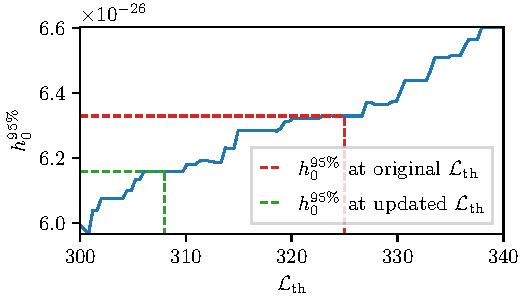
\includegraphics[width=0.8\linewidth]{swift1756_h95_thrange.pdf}
    \caption{Detectable strain $h_0^{95\%}$ as a function of the threshold $\lth$ for the $2f_\star$ subband of Swift J1756.9$-$2508. The original $\lth$ used in the O3 search, and corresponding $h_0^{95\%}$, is marked with a red dashed line. The updated $\lth$ obtained by restricting the search space in $P$--$\tasc$ to only the templates contained within the true joint prior, as shown in Figure~\ref{fig:grid_ellipse}, results in an updated $h_0^{95\%}$, and is marked with a green dashed line.}
    \label{fig:lth_range}
\end{figure}

Combining the five improvements described above allows us to estimate the improvement in sensitivity that we may achieve for a search for continuous gravitational waves from AMXPs using O4 data. Substituting fiducial values we find
\begin{align}
    h_0^{95\%,\,\textrm{O4}} \approx&~ 0.48\ h_0^{95\%,\ \textrm{O3}} 
                                    \left(\frac{1.33}{\textrm{BNS}_{\rm range}^{\rm O4} / \textrm{BNS}_{\rm range}^{\rm O3}}\right)\ 
                                    \left(\frac{1.64}{T_{\rm obs}^{\rm O4} / T_{\rm obs}^{\rm O3}}\right)^{1/4} 
                                    \left(\frac{2}{T_{\rm drift}^{\rm O4} / T_{\rm drift}^{\rm O3}}\right)^{1/4} \nonumber \\ 
                                    &\times \left(\frac{95\%}{\textrm{Search space reduction}}\right)^{-1} 
                                    \left(\frac{90\%}{\textrm{Phase tracking HMM}}\right)^{-1}\,,  \label{eq:h095_improve}
\end{align}
where superscripts of O3 and O4 refer to parameter values in those respective observing runs. The first two terms in parentheses correspond to the improvement in detector sensitivity and the increase in observation duration respectively. The third term corresponds to increasing $T_{\rm drift}$ from 10 to 20\,d. The fourth term arises due to reducing the number of templates, and the effect this has on $\lth$, i.e.~by reducing the trials factor. The fifth term is a rough estimate of the potential benefit from using the HMM scheme described by \citet{Melatos2021}. We find that the fiducial upper limits we set in O4 should improve on the upper limits set in O3 by over a factor of two, increasing our probability of detection. 

If a factor of two is insufficient in producing a detection, we can look to future, even more sensitive detectors such as the Einstein Telescope \citep{Punturo2010} and Cosmic Explorer \citep{ce2017}. These proposed detectors will reduce the single-sided noise power spectral density compared to current LIGO detectors by over an order of magnitude \citep{Punturo2010,ce2017}, thus improving our sensitivity by a factor of $\sim$five. However, these detectors are not yet built or fully funded, and are unlikely to come online before the 2040s. Our best prospects for detecting continuous gravitational waves in the medium-term therefore lie in the factors discussed in Equation~\eqref{eq:h095_improve}: \begin{enumerate*} 
\item improving the sensitivity of current-generation detectors;
\item ingesting longer spans of data, with longer coherence lengths (if the physics allows); and
\item optimizing search algorithms.
\end{enumerate*}